\documentclass[12pt,letterpaper]{article}
\usepackage[utf8]{inputenc}
\usepackage[spanish]{babel}
\usepackage{graphicx}
\usepackage[left=2cm,right=2cm,top=2cm,bottom=2cm]{geometry}
\usepackage{graphicx} % figuras
% \usepackage{subfigure} % subfiguras
\usepackage{float} % para usar [H]
\usepackage{amsmath}
%\usepackage{txfonts}
\usepackage{stackrel} 
\usepackage{multirow}
\usepackage{enumerate} % enumerados
\renewcommand{\labelitemi}{$-$}
\renewcommand{\labelitemii}{$\cdot$}
% \author{}
% \title{Caratula}
\begin{document}

% Fancy Header and Footer
% \usepackage{fancyhdr}
% \pagestyle{fancy}
% \cfoot{}
% \rfoot{\thepage}
%

% \usepackage[hidelinks]{hyperref} % CREA HYPERVINCULOS EN INDICE

% \author{}
\title{Caratula}

\begin{titlepage}
\begin{center}
\large{UNERSIDAD PRIVADA DE TACNA}\\
\vspace*{-0.025in}
\begin{figure}[htb]
\begin{center}

\includegraphics[width=8cm]{./Imagenes/logo}
\end{center}
\end{figure}
\vspace*{0.15in}
INGENIERIA DE SISTEMAS  \\

\vspace*{0.5in}
\begin{large}
TITULO:\\
\end{large}

\vspace*{0.1in}
\begin{Large}
\textbf{INFORME DE LABORATORIO No 01} \\
\end{Large}

\vspace*{0.3in}
\begin{Large}
\textbf{CURSO:} \\
\end{Large}

\vspace*{0.1in}
\begin{large}
BASE DE DATOS II\\
\end{large}

\vspace*{0.3in}
\begin{Large}
\textbf{DOCENTE:} \\
\end{Large}

\vspace*{0.1in}
\begin{large}
Ing.  Patrick Cuadros Quiroga\\
\end{large}

\vspace*{0.2in}
\vspace*{0.1in}
\begin{large}
Integrantes: \\
\begin{flushleft}
Espinoza Caso, Lisbeth		\hfill	(2011040667) \\
...
Continuen poniendo sus nombres
\end{flushleft}
\end{large}
\end{center}

\end{titlepage}


\tableofcontents % INDICE
\thispagestyle{empty} % INDICE SIN NUMERO
\newpage
\setcounter{page}{1} % REINICIAR CONTADOR DE PAGINAS DESPUES DEL INDICE

\section{Actividad No 01 – Revisi\'on de Sintaxis} 
De los siguientes comandos ¿Cuál es el resultado? ¿En caso de ser error cual sería la sentencia correcta?

\begin{itemize}
	\item SELECT last\_name, job\_id, salary AS Sal FROM employees;
	\\Es correcta
	\begin{center}
	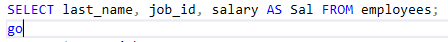
\includegraphics[width=15cm]{./Imagenes/actividad_01_01a} 
	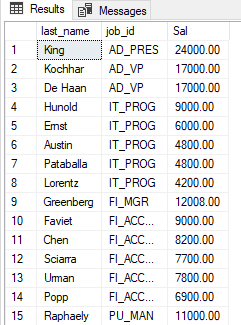
\includegraphics[width=6cm]{./Imagenes/actividad_01_01} 
	\end{center}

	\item SELECT * FROM job\_grades;
	\\Es incorrecta, la sentencia correcta sería:
	\\
	\\SELECT * FROM jobs;
	\begin{center}
	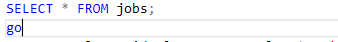
\includegraphics[width=11cm]{./Imagenes/actividad_01_02a} 
	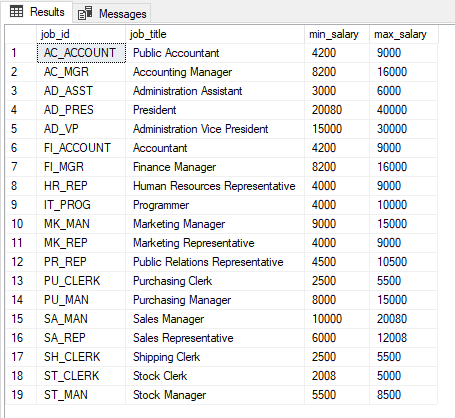
\includegraphics[width=11cm]{./Imagenes/actividad_01_02} 
	\end{center}
	
	\item SELECT employee\_id, last\_name sal x 12 ANNUAL SALARY FROM employees;
	\\Es incorrecta, la sentencia correcta sería:
	\\
	\\SELECT employee\_id, last\_name, salary * 12 'ANNUAL SALARY' FROM employees;
	\begin{center}
	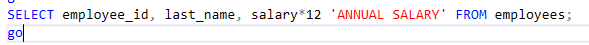
\includegraphics[width=15cm]{./Imagenes/actividad_01_03a} 
	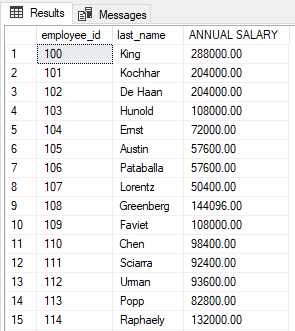
\includegraphics[width=7cm]{./Imagenes/actividad_01_03} 
	\end{center}

\end{itemize} 
\section{Actividad No 02 – Reconociendo la estructura} 

\begin{enumerate}[1.]
	\item Se requiere determinar la estructura de la tabla DEPARTMENTS y sus datos.
	\\
	\\SP\_HELP 'DEPARTMENTS'

	\begin{center}
	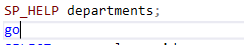
\includegraphics[width=9cm]{./Imagenes/actividad_02_01a} 
	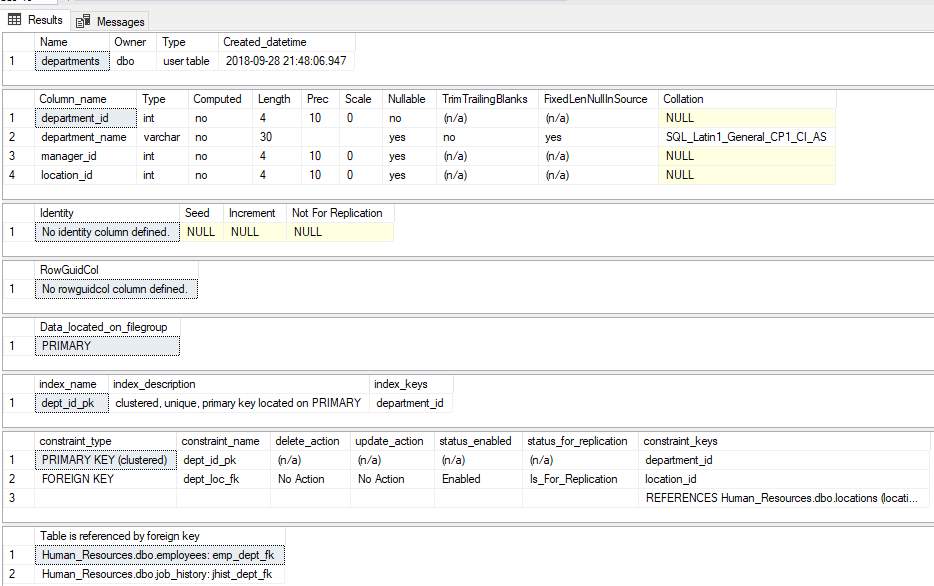
\includegraphics[width=15cm]{./Imagenes/actividad_02_01} 
	\end{center}

	\item El departamento de Recursos Humanos requiere un reporte que muestre los campos: employee\_id, last\_name y job\_id, asicomo el campo hire\_date con el alias StartDate.
	\\
	\\SELECT emp.employee\_id, \\
	emp.last\_name, \\
	emp.job\_id, \\
	emp.hire\_date AS StartDate \\
	FROM employees AS emp; 

	\begin{center}
	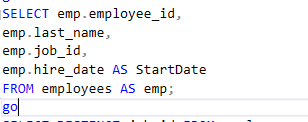
\includegraphics[width=10cm]{./Imagenes/actividad_02_02a} 
	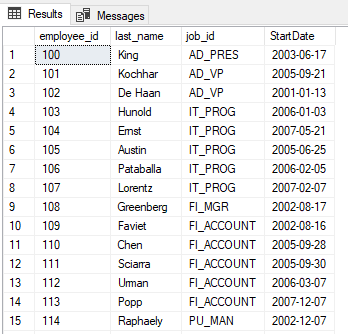
\includegraphics[width=10cm]{./Imagenes/actividad_02_02} 
	\end{center}

	\item Finalmente el departamento de Recursos Humanos requiere un listado de todos valores del campo JOB\_ID de la tabla EMPLOYEES pero que se muestren de forma única y no repetida.
	\\
	\\SELECT DISTINCT job\_id FROM employees; 

	\begin{center}
	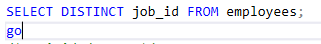
\includegraphics[width=11cm]{./Imagenes/actividad_02_03a} 
	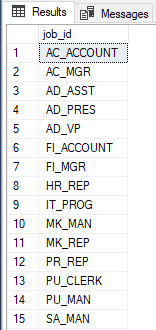
\includegraphics[width=6cm]{./Imagenes/actividad_02_03} 
	\end{center}

\end{enumerate}



\section{Actividad No 03 – Consultas B\'asicas} 
		
\begin{enumerate}[1.]
	\item El departamento de Recursos Humanos requiere ampliar el reporte anterior (4.2.2) para hacerlo m\'as comprensible, por lo que se requiere que los encabezados de las columnas sean: Emp No, Empleado, Puesto y Fecha Contrataci\'on.
	\\
	\\SELECT emp.employee\_id AS 'Emp N', \\
	   emp.last\_name AS Empleado, \\
	   emp.job\_id AS Puesto, \\
	   emp.hire\_date AS 'Fecha de contrataci\'on' \\
	FROM employees AS emp; \\
	\begin{center}
	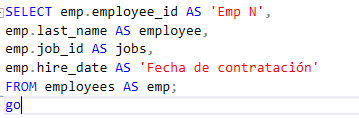
\includegraphics[width=9cm]{./Imagenes/actividad_03_01a} 
	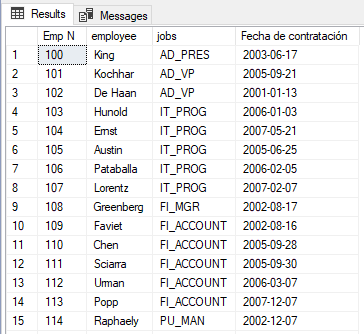
\includegraphics[width=10cm]{./Imagenes/actividad_03_01} 
	\end{center}

	\item Adicionalmente el departamento de Recursos Humanos requiere un reporte más sencillo, en el que se muestre los campos: last\_name y job\_id en una sola y \'unica columna (los datos deben estar separados por una coma) que tenga como alias Empleado y Puesto.
	\\
	\\SELECT CONCAT(emp.last\_name,',',emp.job\_id) AS 'Empleado y Puesto' \\
	\\FROM employees AS emp; \\
	\begin{center}
	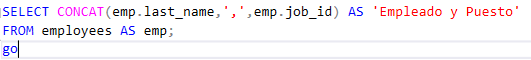
\includegraphics[width=13cm]{./Imagenes/actividad_03_02a}
	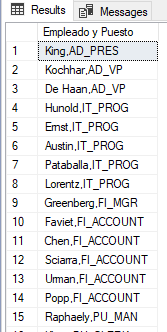
\includegraphics[width=5cm]{./Imagenes/actividad_03_02} 
	\end{center}

	\item Finalmente a modo de práctica, realizar una consulta que muestre todos los campos de la tabla EMPLOYEES, en una sola y única columna, los datos deben estar separados por una coma y la columna debe tener como encabezado Los Empleados
	\\
	\\SELECT CONCAT(emp.employee\_id,',', \\
			  emp.first\_name,',', \\
			  emp.last\_name,',', \\
			  emp.email,',', \\
			  emp.phone\_number,',', \\
			  emp.hire\_date,',', \\
			  emp.job\_id,',', \\
			  emp.salary,',', \\
			  emp.commission\_pct,',', \\
			  emp.manager\_id,',', \\
			  emp.department\_id) AS 'Los empleados' \\
	FROM employees AS emp; \\
	\begin{center}
	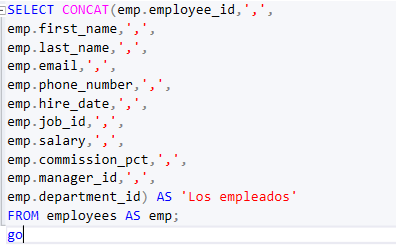
\includegraphics[width=9cm]{./Imagenes/actividad_03_03a}
	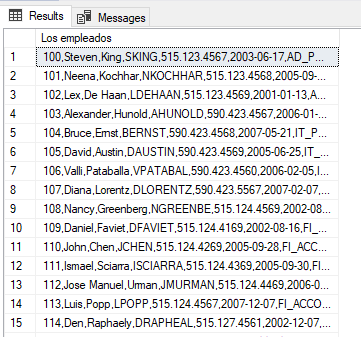
\includegraphics[width=11cm]{./Imagenes/actividad_03_03}
	\end{center}

\end{enumerate}




\section{Actividad No 04 – Restricci\'on y Ordenamiento} 
		
\begin{enumerate}[1.]
	\item Debido a problemas con el presupuesto, el departamento de Recursos Humanos requiere un reporte que muestre los apellidos (last\_name) y salarios (salary) de todos los empleados que ganen más de \$ 12,000.
	\\ \\ select last\_name,salary from employees where salary > 12000;

	\begin{center}
	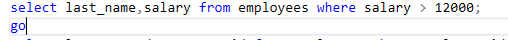
\includegraphics[width=5cm]{./Imagenes/actividad_04_01a} 
	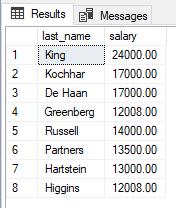
\includegraphics[width=5cm]{./Imagenes/actividad_04_01} 
	\end{center}

	\item Asimismo se requiere realizar una consulta que muestre los apellidos (last\_name) y el n\'umero de departamento (department\_id) para los empleados que tengan numero (employee\_id) 176.
	\\ \\select last\_name,department\_id from employees where employee\_id > 176;

	\begin{center}
	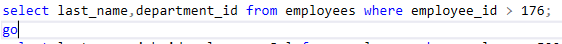
\includegraphics[width=5cm]{./Imagenes/actividad_04_02a}
	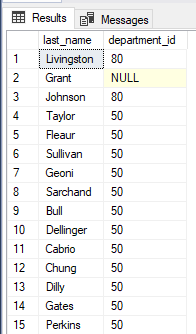
\includegraphics[width=5cm]{./Imagenes/actividad_04_02} 
	\end{center}

	\item El departamento de Recursos Humanos necesita determinar los mayores y menores sueldos, modificar la consulta del  ítem 4.1. para mostrar el apellido y salario de cada empleado cuyo sueldo no est\'e en el rango de \$ 5,000 a \$ 12,000.
	\\ \\select last\_name,job\_id,salary as Sal from employees where salary > 5000 and salary < 12000;

	\begin{center}
	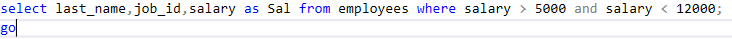
\includegraphics[width=5cm]{./Imagenes/actividad_04_03a} 
	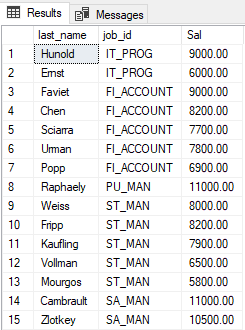
\includegraphics[width=5cm]{./Imagenes/actividad_04_03} 
	\end{center}

	\item Crear un reporte que muestre los apellidos (last\_name), puesto (job\_id) y fecha de contrataci\'on (hire\_date), de los empleados que apellidan ‘Matos’ y ‘Taylor’, asimismo presentar el reporte ordenado ascendentemente por fecha de contrataci\'on.
	\\ \\select last\_name,job\_id,hire\_date from employees where last\_name = 'Matos' or last\_name = 'Taylor' order by hire\_date asc;

	\begin{center}
	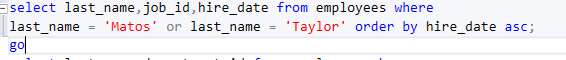
\includegraphics[width=5cm]{./Imagenes/actividad_04_04a} 
	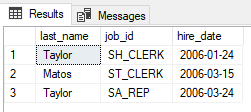
\includegraphics[width=5cm]{./Imagenes/actividad_04_04} 
	\end{center}

	\item Mostrar los apellidos (last\_name) y n\'umero de departamento (departamento\_id) de todos los empleados que pertenezcan a los departamentos 20 o 50 en orden alfab\'etico ascendente por el apellido.
	\\ \\select last\_name,department\_id from employees where department\_id = 20 or department\_id = 50 order by last\_name asc;
	
	\begin{center}
	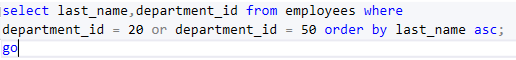
\includegraphics[width=5cm]{./Imagenes/actividad_04_05a}
	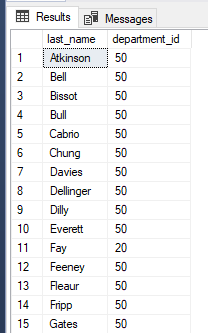
\includegraphics[width=5cm]{./Imagenes/actividad_04_05} 
	\end{center}
	
	\item Modificar el reporte del ítem 4.1. para mostrar los apellidos y salarios de los empleados que tengan un salario entre los \$ 5,000 a \$ 12,000 y pertenezcan a los números de departamento 20 o 50. Asimismo etiquetar las cabeceras de los resultados con los alias Empleado y Salario Mensual respectivamente.
	\\ \\select last\_name 'Empleado',salary 'Salario Mensual' from employees where salary > 5000 and salary < 12000 and (department\_id = 20 or department\_id = 50);

	\begin{center}
	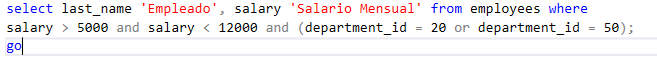
\includegraphics[width=5cm]{./Imagenes/actividad_04_06a}
	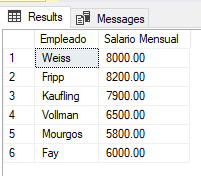
\includegraphics[width=5cm]{./Imagenes/actividad_04_06} 
	\end{center}

	\item El departamento de Recursos Humanos necesita un listado de apellidos (last\_name) y fecha de contrataci\'on (hire\_date) de todos los empleados que fueron contratados el año 1994.
	\\ \\select last\_name,hire\_date from employees where hire\_date between '19940101' and '19941231';

	\begin{center}
	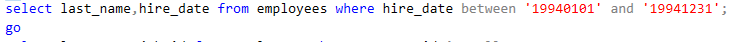
\includegraphics[width=5cm]{./Imagenes/actividad_04_07a}
	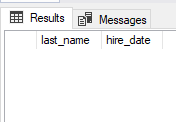
\includegraphics[width=5cm]{./Imagenes/actividad_04_07} 
	\end{center}

	\item Crear un reporte que muestre los apellidos (last\_name) y puesto (job\_id) de todos los empleados que no tengan un administrador (manager).
	\\ \\select last\_name,job\_id from employees where manager\_id is null;

	\begin{center}
	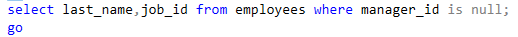
\includegraphics[width=5cm]{./Imagenes/actividad_04_08a} 
	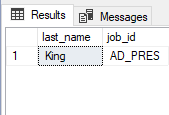
\includegraphics[width=5cm]{./Imagenes/actividad_04_08} 
	\end{center}

	\item Crear un reporte para mostrar los apellidos (last\_name), salario (salary) y \% de comisión (commission\_pct). Ordenar los datos por salario y comisión de manera descendente, utilizar la opción numérica de la cláusula ORDER BY.
	\\ \\select last\_name,salary,commission\_pct from employees order by salary desc,commission\_pct desc;

	\begin{center}
	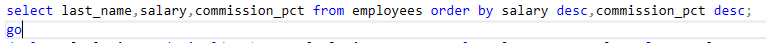
\includegraphics[width=5cm]{./Imagenes/actividad_04_09a} 
	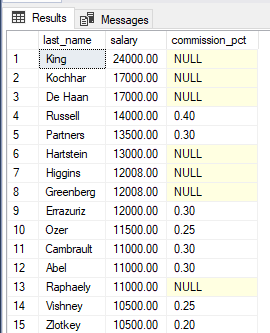
\includegraphics[width=5cm]{./Imagenes/actividad_04_09} 
	\end{center}


	\item El personal del departamento de Recursos Humanos desea tener mayor flexibilidad con los reportes hechos. Por ejemplo se requiere un reporte de los apellidos (last\_name) y salarios (salary) de todos los empleados que tengan un salario mayor a un monto que el personal de Recursos Humanos ingresará. Probar con el valor \$ 12,000.
	\\ \\declare @salario as decimal(9,2); set @salario = 12000; select last\_name,salary from employees where salary > @salario;

	\begin{center}
	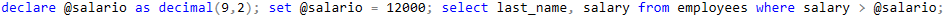
\includegraphics[width=5cm]{./Imagenes/actividad_04_10a} 
	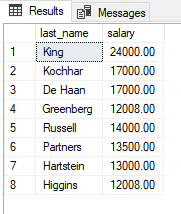
\includegraphics[width=5cm]{./Imagenes/actividad_04_10} 
	\end{center}

	\item El departamento de Recursos Humanos requiere extraer reporte basados en el Administrador (manager\_id). Se requiere crear una consulta que pregunte al usuario por el Administrador (manager\_id) y genere un reporte con los números de empleado (employee\_id), apellidos (last\_name), salarios (salary) y numero de departamento de los empleados que este Administrador tiene a su cargo. Adicionalmente también se desea tener la habilidad de ordenar este reporte en base a una determinada columna. Probar con los siguientes valores:
	\\Administrador (manager\_id) = 103, ordenado por Apellido (last\_name)
	\\Administrador (manager\_id) = 201, ordenado por Salario (salary)
	\\Administrador (manager\_id) = 124, ordenado por No de Empleado (employee\_id)
	\\ \\declare @gerente as int;
	\\set @gerente = 103;
	\\select employee\_id,last\_name,salary,department\_id from employees where manager\_id = @gerente order by last\_name;
	\\set @gerente = 201;
	\\select employee\_id,last\_name,salary,department\_id from employees where manager\_id = @gerente order by salary;
	\\set @gerente = 124;
	\\select employee\_id,last\_name,salary,department\_id from employees where manager\_id = @gerente order by employee\_id;
	\\go
	
	\begin{center}
	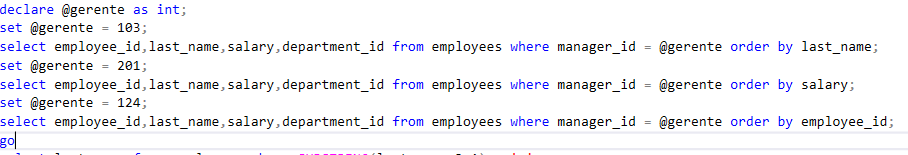
\includegraphics[width=5cm]{./Imagenes/actividad_04_11a} 
	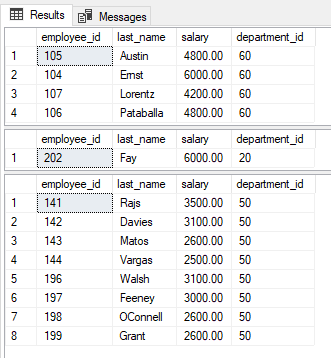
\includegraphics[width=5cm]{./Imagenes/actividad_04_11} 
	\end{center}

	\item Generar un listado de apellidos (last\_name) de todos los empleados que tengan la letra ‘a’ en la tercera letra de su apellido.
	\\ \\select last\_name from employees where SUBSTRING(last\_name,3,1) = 'a';
	\\go

	\begin{center}
	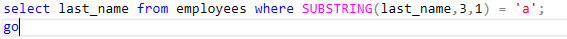
\includegraphics[width=5cm]{./Imagenes/actividad_04_12a} 
	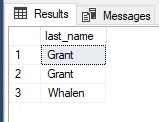
\includegraphics[width=5cm]{./Imagenes/actividad_04_12} 
	\end{center}

	\item Mostrar los apellidos (last\_name) de todos los empleados que tengan tanto la letra ‘a’ como la letra ‘e’ en su apellido.
	\\ \\select last\_name from employees where SUBSTRING(last\_name,3,1) = 'a' or SUBSTRING(last\_name,3,1) = 'e';
	\\go

	\begin{center}
	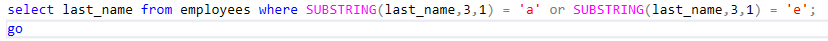
\includegraphics[width=5cm]{./Imagenes/actividad_04_13a} 
	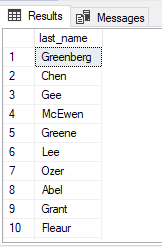
\includegraphics[width=5cm]{./Imagenes/actividad_04_13} 
	\end{center}

	\item Mostrar los apellidos (last\_name), puestos (job\_id) y salario (salary) de todos los empleados que sean Representantes de Ventas (SA\_REP) o Responsables de Inventario (ST\_CLERK) y cuyos salarios no sean iguales a \$ 2,500, \$ 3,500 o \$ 7,000.
	\\ \\select last\_name,job\_id,salary from employees where (job\_id = 'SA\_REP' or job\_id = 'ST\_CLERK') and (salary = 2500 or salary = 3500 or salary = 7000);
	\\go

	\begin{center}
	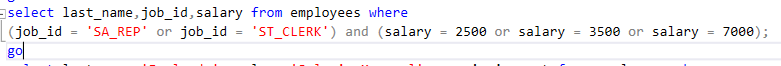
\includegraphics[width=5cm]{./Imagenes/actividad_04_14a} 
	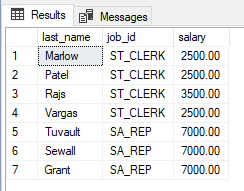
\includegraphics[width=5cm]{./Imagenes/actividad_04_14} 
	\end{center}

	\item Modificar el reporte del ítem 4.6 y mostrar adicionalmente los datos de comisión (commission\_pct) de todos los empleados que solamente el 20\% de comisi\'on.
	\\ \\select last\_name 'Empleado',salary 'Salario Mensual',commission\_pct from employees where salary > 5000 and salary < 12000 and (department\_id = 20 or department\_id = 50) and commission\_pct = 0.20;
	\\go

	\begin{center}
	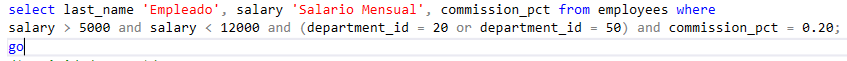
\includegraphics[width=5cm]{./Imagenes/actividad_04_15a} 
	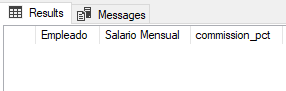
\includegraphics[width=5cm]{./Imagenes/actividad_04_15} 
	\end{center}

\end{enumerate}


\section{Actividad No 05 – Funciones}
	
\begin{enumerate}[1.]
	\item Se requiere realizar una consulta que visualice la fecha del sistema.
	\\
	\\SELECT CONVERT (date, SYSDATETIME())
	\\,CONVERT (date, SYSDATETIMEOFFSET())
	\\,CONVERT (date, SYSUTCDATETIME())
	\\,CONVERT (date, CURRENT\_TIMESTAMP)
	\\,CONVERT (date, GETDATE())
    	\\,CONVERT (date, GETUTCDATE());
	\begin{center}
	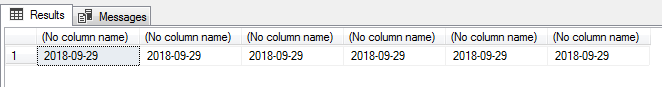
\includegraphics[width=5cm]{./Imagenes/actividad_05_01}
	\end{center}
	
	\item El departamento de Recursos Humanos necesita un reporte de todos los empleados que muestre el No de Empleado, Apellidos, Salario y una columna más con el cálculo del salario incrementado en 15.5\% (expresado solo en enteros) esta columna debe etiquetarse Nuevo Salario
	\\
	\\SELECT employee\_id,last\_name,salary,salary*0.155 as newsalary FROM employees
	\begin{center}
	\includegraphics[width=5cm]{./Imagenes/actividad_05_02}
	\end{center}

	\item Modificar la consulta anterior y adicionar una columna que muestre el resultado de la resta entre el antiguo salario y el nuevo salario. Etiquetar esta columna como Incremento.
	\\
	\\SELECT employee\_id,last\_name,salary,salary*0.155 as newsalary,salary-(salary*0.155) as incremento FROM employees
	\begin{center}
	\includegraphics[width=5cm]{./Imagenes/actividad_05_03}
	\end{center}

	\item Crear un reporte que muestre los Apellidos (con la primera letra en May\'usculas y las demás en Min\'usculas) y la longitud de los apellidos (colocar alias Longitud), para todos aquellos empleados quienes sus apellidos empiecen con las letras ‘J’, ‘A’ y ‘M’. Ordenar los resultados por la columna Apellido.
	\\
	\\select UPPER(last\_name) "Apellido", (LOWER(first\_name)) "Longitud" 
	\\from employees 
	\\where last\_name like 'A\%'
     	\\ or last\_name like 'J\%'
      	\\or last\_name like 'M\%' order by last\_name asc;
      	\begin{center}
	\includegraphics[width=5cm]{./Imagenes/actividad_05_04}
	\end{center}

	\item Modificar la consulta anterior a fin de que consulte primero al usuario con que letra empieza el apellido a buscar. Considerar que no importa si la letra esta may\'uscula o min\'uscula de igual manera debe mostrar los resultados.
	\\
	\\select initcap(FIRST\_NAME) as "name", length(first\_name) as "Length" from employees where upper(substr(first\_name,1,1))=upper('\&Inicial') order by first\_name;

	\item El departamento de Recursos Humanos la duración o tiempo de permanencia de cada empleado, mostrar el Apellido y el calculo del número de meses entre la fecha de hoy y la fecha en que fue contratado el empleado, Etiquetar la columna como Meses Trabajados, ordenar los resultados por el resultado de los n\'umeros de meses, Redondear el número de meses al entero más cercano.
	\\
	\\SELECT LAST\_NAME, ROUND(MONTHS\_BETWEEN(SYSDATE,HIRE\_DATE),0) "MONTHS\_WORKED"
	\\from employees order by MONTHS\_BETWEEN( HIRE\_DATE, SYSDATE);

	\item Crear una consulta que devuelva los Apellidos y Salarios de todos los empleados, Formatear la columna salario para que muestre 15 caracteres, completar con el símbolo ‘\$’ los espacios previos al valor de la columna salario, ejemplo: \$\$\$\$\$\$\$\$\$\$10000. Etiquetar esta columna como Salario.
	\\
	\\CREATE FUNCTION LPAD
	\\(
	\\ @string VARCHAR(MAX), 
	\\@length INT,          
	\\@pad CHAR             
	\\)
	\\RETURNS VARCHAR(MAX)
	\\AS
	\\BEGIN
	    \\RETURN REPLICATE(@pad, @length - LEN(@string)) + @string;
	\\END
	\\GO
	\\SELECT dbo.LPAD(salary, 15, '\$') VALUE
	\\FROM employees;
	\begin{center}
		\includegraphics[width=5cm]{./Imagenes/actividad_05_07}
	\end{center}

	\item Crear una consulta que muestre en una única columna los primeros 8 caracteres del apellido de los empleados e indique sus salarios representados por asteriscos (‘*’), cada asterisco representa el valor 1000. Ordenar el listado por el salario de los empleados. Asimismo Etiquetar la columna como ‘Empleados y sus Salarios’.
	\item Finalmente crear una consulta que muestre los Apellidos de los empleados y el No de Semanas Empleado hasta la actualidad para todos los empleados del departamento No 90, truncar el número de semanas a sin decimales. Ordenar el resultado por el No de Semanas y etiquetar la columna como tenencia.
	\\
	\\select last\_name, TRUNC(((SYSDATE-hire\_date)/7),0) as TENURE from employees where department\_id=90 ORDER BY hire\_date DESC;
\end{enumerate}


\section{Actividad No 06 – Funciones de Conversi\'on} 
		
\begin{enumerate}[1.]
	\item Crear un reporte que muestre lo siguiente por cada empleado.
	\\(Apellido del empleado) gana (Salario) pero quisiera (3 veces Salario).
	\\Etiquetar la columna como Sueldos Soñados.
	\\
	\\select 'Sueldos Soñados'=(last\_name + ' gana ' + Cast(salary as varchar(18)) + ' pero 
	\\quisiera ' + Cast((salary * 3) as varchar(18))) 
	\\from dbo.employees
	\\go
	\\
	\begin{center}
	\includegraphics[width=15cm]{./Imagenes/actividad_06_01a}
	\includegraphics[width=8cm]{./Imagenes/actividad_06_01}
	\end{center}

	\item Realizar una consulta que muestre el Apellido del empleado, fecha de contratación y la Fecha de Revisión del Salario, la cual es el primer Lunes después de cada seis meses de servicio, etiquetar la columna como Revisión, asimismo el formato de esta fecha debe ser similar al siguiente: 
	\begin{center}
	Lunes, el veintiuno de julio, 2003 
	\end{center}
\
	\\select last\_name, hire\_date as Revision from employees 
	\\where hire\_date between '2003-06-17' and '2005-09-21';
	\\go
	
	\begin{center}
	\includegraphics[width=14cm]{./Imagenes/actividad_06_02a}
	\includegraphics[width=5cm]{./Imagenes/actividad_06_02}
	\end{center}

	\item Mostrar un reporte que tenga los Apellidos, Fecha de Contrataci\'on y el D\'ia de Inicio de cada empleado (Lunes, Martes, etc…), etiquetar la \'ultima columna como D\'ia. Ordenar los resultados por el D\'ia de Inicio empezando por Lunes.
	\\
	\\select e.last\_name, e.hire\_date, DateName(WEEKDAY, jh.START\_DATE)as 'Dia' 
	\\from dbo.employees as e inner join dbo.job\_history as jh on 
	\\e.employee\_id=jh.employee\_id
	\\go
	\\
	\begin{center}
	\includegraphics[width=15cm]{./Imagenes/actividad_06_03a}
	\includegraphics[width=7cm]{./Imagenes/actividad_06_03}
	\end{center}


	\item Crear un listado que muestre los Apellidos de los empleados y sus Montos de Comisi\'on, en caso no tenga comisi\'on deber\'a mostrar el texto ‘Sin Comisi\'on’, etiquetar esta ultima columna como Comisi\'on.
	\\
	\\Sintaxis y demostracion
	\begin{center}
	\includegraphics[width=16cm]{./Imagenes/64}
	\includegraphics[width=7cm]{./Imagenes/642}
	\end{center}


	\item Rescribir la consulta anterior utilizando la función CASE.
	\\
	\\Sintaxis y demostracion
	\begin{center}
	\includegraphics[width=16cm]{./Imagenes/66}
	\includegraphics[width=7cm]{./Imagenes/662}
	\end{center}

\end{enumerate}



\end{document}
